\documentclass[border=14pt,tikz]{standalone}
\usepackage{fontspec}
\setmainfont{Helvetica Neue}
\setsansfont{Helvetica Neue}
\setmonofont{Menlo}
\usepackage{amsmath}
\usepackage{tikz}
\usetikzlibrary{positioning, arrows.meta}

\definecolor{kernel}{HTML}{E3F2FD}
\definecolor{kernelborder}{HTML}{2196F3}
\definecolor{state}{HTML}{E8F5E9}
\definecolor{stateborder}{HTML}{4CAF50}
\definecolor{choice}{HTML}{FFF3E0}
\definecolor{choiceborder}{HTML}{FF9800}

\begin{document}
\pagecolor{white}
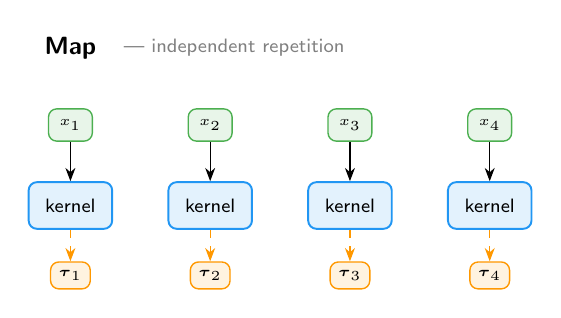
\begin{tikzpicture}[
    >=Stealth,
    node distance=0.8cm and 1.2cm,
    kern/.style={draw, rounded corners=3pt, inner sep=6pt,
                 font=\sffamily\scriptsize, fill=kernel, draw=kernelborder, line width=0.7pt},
    st/.style={draw, rounded corners=3pt, inner sep=4pt,
               font=\ttfamily\tiny, fill=state, draw=stateborder, line width=0.5pt},
    ch/.style={draw, rounded corners=3pt, inner sep=3pt,
               font=\ttfamily\tiny, fill=choice, draw=choiceborder, line width=0.5pt},
    title/.style={font=\sffamily\small\bfseries},
    annot/.style={font=\sffamily\scriptsize, text=black!50},
]

\node[title] (mt) {Map};
\node[annot, right=3pt of mt] {--- independent repetition};

\node[st, below=0.5cm of mt] (x1) {$x_1$};
\node[st, right=of x1] (x2) {$x_2$};
\node[st, right=of x2] (x3) {$x_3$};
\node[st, right=of x3] (x4) {$x_4$};

\node[kern, below=0.5cm of x1] (m1) {kernel};
\node[kern, below=0.5cm of x2] (m2) {kernel};
\node[kern, below=0.5cm of x3] (m3) {kernel};
\node[kern, below=0.5cm of x4] (m4) {kernel};

\draw[->] (x1) -- (m1);
\draw[->] (x2) -- (m2);
\draw[->] (x3) -- (m3);
\draw[->] (x4) -- (m4);

\node[ch, below=0.4cm of m1] (mc1) {$\boldsymbol{\tau}_1$};
\node[ch, below=0.4cm of m2] (mc2) {$\boldsymbol{\tau}_2$};
\node[ch, below=0.4cm of m3] (mc3) {$\boldsymbol{\tau}_3$};
\node[ch, below=0.4cm of m4] (mc4) {$\boldsymbol{\tau}_4$};
\draw[->, dashed, choiceborder] (m1) -- (mc1);
\draw[->, dashed, choiceborder] (m2) -- (mc2);
\draw[->, dashed, choiceborder] (m3) -- (mc3);
\draw[->, dashed, choiceborder] (m4) -- (mc4);

\end{tikzpicture}
\end{document}
